% Options for packages loaded elsewhere
\PassOptionsToPackage{unicode}{hyperref}
\PassOptionsToPackage{hyphens}{url}
%
\documentclass[
]{article}
\title{Projeto final}
\author{Diego}
\date{3/12/2022}

\usepackage{amsmath,amssymb}
\usepackage{lmodern}
\usepackage{iftex}
\ifPDFTeX
  \usepackage[T1]{fontenc}
  \usepackage[utf8]{inputenc}
  \usepackage{textcomp} % provide euro and other symbols
\else % if luatex or xetex
  \usepackage{unicode-math}
  \defaultfontfeatures{Scale=MatchLowercase}
  \defaultfontfeatures[\rmfamily]{Ligatures=TeX,Scale=1}
\fi
% Use upquote if available, for straight quotes in verbatim environments
\IfFileExists{upquote.sty}{\usepackage{upquote}}{}
\IfFileExists{microtype.sty}{% use microtype if available
  \usepackage[]{microtype}
  \UseMicrotypeSet[protrusion]{basicmath} % disable protrusion for tt fonts
}{}
\makeatletter
\@ifundefined{KOMAClassName}{% if non-KOMA class
  \IfFileExists{parskip.sty}{%
    \usepackage{parskip}
  }{% else
    \setlength{\parindent}{0pt}
    \setlength{\parskip}{6pt plus 2pt minus 1pt}}
}{% if KOMA class
  \KOMAoptions{parskip=half}}
\makeatother
\usepackage{xcolor}
\IfFileExists{xurl.sty}{\usepackage{xurl}}{} % add URL line breaks if available
\IfFileExists{bookmark.sty}{\usepackage{bookmark}}{\usepackage{hyperref}}
\hypersetup{
  pdftitle={Projeto final},
  pdfauthor={Diego},
  hidelinks,
  pdfcreator={LaTeX via pandoc}}
\urlstyle{same} % disable monospaced font for URLs
\usepackage[margin=1in]{geometry}
\usepackage{color}
\usepackage{fancyvrb}
\newcommand{\VerbBar}{|}
\newcommand{\VERB}{\Verb[commandchars=\\\{\}]}
\DefineVerbatimEnvironment{Highlighting}{Verbatim}{commandchars=\\\{\}}
% Add ',fontsize=\small' for more characters per line
\usepackage{framed}
\definecolor{shadecolor}{RGB}{248,248,248}
\newenvironment{Shaded}{\begin{snugshade}}{\end{snugshade}}
\newcommand{\AlertTok}[1]{\textcolor[rgb]{0.94,0.16,0.16}{#1}}
\newcommand{\AnnotationTok}[1]{\textcolor[rgb]{0.56,0.35,0.01}{\textbf{\textit{#1}}}}
\newcommand{\AttributeTok}[1]{\textcolor[rgb]{0.77,0.63,0.00}{#1}}
\newcommand{\BaseNTok}[1]{\textcolor[rgb]{0.00,0.00,0.81}{#1}}
\newcommand{\BuiltInTok}[1]{#1}
\newcommand{\CharTok}[1]{\textcolor[rgb]{0.31,0.60,0.02}{#1}}
\newcommand{\CommentTok}[1]{\textcolor[rgb]{0.56,0.35,0.01}{\textit{#1}}}
\newcommand{\CommentVarTok}[1]{\textcolor[rgb]{0.56,0.35,0.01}{\textbf{\textit{#1}}}}
\newcommand{\ConstantTok}[1]{\textcolor[rgb]{0.00,0.00,0.00}{#1}}
\newcommand{\ControlFlowTok}[1]{\textcolor[rgb]{0.13,0.29,0.53}{\textbf{#1}}}
\newcommand{\DataTypeTok}[1]{\textcolor[rgb]{0.13,0.29,0.53}{#1}}
\newcommand{\DecValTok}[1]{\textcolor[rgb]{0.00,0.00,0.81}{#1}}
\newcommand{\DocumentationTok}[1]{\textcolor[rgb]{0.56,0.35,0.01}{\textbf{\textit{#1}}}}
\newcommand{\ErrorTok}[1]{\textcolor[rgb]{0.64,0.00,0.00}{\textbf{#1}}}
\newcommand{\ExtensionTok}[1]{#1}
\newcommand{\FloatTok}[1]{\textcolor[rgb]{0.00,0.00,0.81}{#1}}
\newcommand{\FunctionTok}[1]{\textcolor[rgb]{0.00,0.00,0.00}{#1}}
\newcommand{\ImportTok}[1]{#1}
\newcommand{\InformationTok}[1]{\textcolor[rgb]{0.56,0.35,0.01}{\textbf{\textit{#1}}}}
\newcommand{\KeywordTok}[1]{\textcolor[rgb]{0.13,0.29,0.53}{\textbf{#1}}}
\newcommand{\NormalTok}[1]{#1}
\newcommand{\OperatorTok}[1]{\textcolor[rgb]{0.81,0.36,0.00}{\textbf{#1}}}
\newcommand{\OtherTok}[1]{\textcolor[rgb]{0.56,0.35,0.01}{#1}}
\newcommand{\PreprocessorTok}[1]{\textcolor[rgb]{0.56,0.35,0.01}{\textit{#1}}}
\newcommand{\RegionMarkerTok}[1]{#1}
\newcommand{\SpecialCharTok}[1]{\textcolor[rgb]{0.00,0.00,0.00}{#1}}
\newcommand{\SpecialStringTok}[1]{\textcolor[rgb]{0.31,0.60,0.02}{#1}}
\newcommand{\StringTok}[1]{\textcolor[rgb]{0.31,0.60,0.02}{#1}}
\newcommand{\VariableTok}[1]{\textcolor[rgb]{0.00,0.00,0.00}{#1}}
\newcommand{\VerbatimStringTok}[1]{\textcolor[rgb]{0.31,0.60,0.02}{#1}}
\newcommand{\WarningTok}[1]{\textcolor[rgb]{0.56,0.35,0.01}{\textbf{\textit{#1}}}}
\usepackage{graphicx}
\makeatletter
\def\maxwidth{\ifdim\Gin@nat@width>\linewidth\linewidth\else\Gin@nat@width\fi}
\def\maxheight{\ifdim\Gin@nat@height>\textheight\textheight\else\Gin@nat@height\fi}
\makeatother
% Scale images if necessary, so that they will not overflow the page
% margins by default, and it is still possible to overwrite the defaults
% using explicit options in \includegraphics[width, height, ...]{}
\setkeys{Gin}{width=\maxwidth,height=\maxheight,keepaspectratio}
% Set default figure placement to htbp
\makeatletter
\def\fps@figure{htbp}
\makeatother
\setlength{\emergencystretch}{3em} % prevent overfull lines
\providecommand{\tightlist}{%
  \setlength{\itemsep}{0pt}\setlength{\parskip}{0pt}}
\setcounter{secnumdepth}{-\maxdimen} % remove section numbering
\ifLuaTeX
  \usepackage{selnolig}  % disable illegal ligatures
\fi

\begin{document}
\maketitle

\hypertarget{section}{%
\section{}\label{section}}

\begin{Shaded}
\begin{Highlighting}[]
\NormalTok{stocks }\OtherTok{\textless{}{-}} \FunctionTok{c}\NormalTok{(}\StringTok{"ibov3"}\NormalTok{, }\StringTok{"ENBR3"}\NormalTok{, }\StringTok{""}\NormalTok{)}

\CommentTok{\# "VALE3.SA",}
\NormalTok{my\_stocks }\OtherTok{\textless{}{-}} \FunctionTok{c}\NormalTok{(}\StringTok{"ITUB3.SA"}\NormalTok{, }\StringTok{"ENBR3.SA"}\NormalTok{,}
               \StringTok{"FLRY3.SA"}\NormalTok{, }\StringTok{"B3SA3.SA"}\NormalTok{, }\StringTok{"BBDC3.SA"}\NormalTok{,}
               \StringTok{"EGIE3.SA"}\NormalTok{, }\StringTok{"TAEE11.SA"}\NormalTok{, }\StringTok{"WEGE3.SA"}\NormalTok{, }
               \StringTok{"PSSA3.SA"}
\NormalTok{               )}

\NormalTok{asset\_returns }\OtherTok{\textless{}{-}} 
  \FunctionTok{BatchGetSymbols}\NormalTok{(my\_stocks,}
                \AttributeTok{first.date =} \StringTok{"2000{-}01{-}01"}\NormalTok{,}
                \AttributeTok{bench.ticker =} \StringTok{"\^{}BVSP"}\NormalTok{,}
                \AttributeTok{type.return =} \StringTok{"log"}
\NormalTok{                )}\SpecialCharTok{$}\NormalTok{df.tickers }\SpecialCharTok{\%\textgreater{}\%} 
  \FunctionTok{select}\NormalTok{(ref.date, ticker, ret.closing.prices, price.close) }\SpecialCharTok{\%\textgreater{}\%} 
  \FunctionTok{na.omit}\NormalTok{()}
\end{Highlighting}
\end{Shaded}

\begin{verbatim}
## 
## Running BatchGetSymbols for:
##    tickers =ITUB3.SA, ENBR3.SA, FLRY3.SA, B3SA3.SA, BBDC3.SA, EGIE3.SA, TAEE11.SA, WEGE3.SA, PSSA3.SA
##    Downloading data for benchmark ticker
## ^BVSP | yahoo (1|1) | Not Cached | Saving cache
## ITUB3.SA | yahoo (1|9) | Not Cached | Saving cache - Got 100% of valid prices | Looking good!
## ENBR3.SA | yahoo (2|9) | Not Cached | Saving cache - Got 100% of valid prices | Good job!
## FLRY3.SA | yahoo (3|9) | Not Cached | Saving cache - Got 55% of valid prices | OUT: not enough data (thresh.bad.data = 75%)
## B3SA3.SA | yahoo (4|9) | Not Cached | Saving cache - Got 65% of valid prices | OUT: not enough data (thresh.bad.data = 75%)
## BBDC3.SA | yahoo (5|9) | Not Cached | Saving cache - Got 100% of valid prices | You got it!
## EGIE3.SA | yahoo (6|9) | Not Cached | Saving cache - Got 90% of valid prices | Nice!
## TAEE11.SA | yahoo (7|9) | Not Cached | Saving cache - Got 64% of valid prices | OUT: not enough data (thresh.bad.data = 75%)
## WEGE3.SA | yahoo (8|9) | Not Cached | Saving cache - Got 100% of valid prices | Youre doing good!
## PSSA3.SA | yahoo (9|9) | Not Cached | Saving cache - Got 78% of valid prices | Got it!
\end{verbatim}

\begin{Shaded}
\begin{Highlighting}[]
\NormalTok{asset\_returns }\SpecialCharTok{\%\textgreater{}\%} 
  \FunctionTok{group\_by}\NormalTok{(ticker) }\SpecialCharTok{\%\textgreater{}\%} 
  \FunctionTok{count}\NormalTok{()}
\end{Highlighting}
\end{Shaded}

\begin{verbatim}
## # A tibble: 6 x 2
## # Groups:   ticker [6]
##   ticker       n
##   <chr>    <int>
## 1 BBDC3.SA  5575
## 2 EGIE3.SA  5011
## 3 ENBR3.SA  5569
## 4 ITUB3.SA  5575
## 5 PSSA3.SA  4301
## 6 WEGE3.SA  5575
\end{verbatim}

\begin{Shaded}
\begin{Highlighting}[]
\NormalTok{plot\_returns }\OtherTok{\textless{}{-}} \ControlFlowTok{function}\NormalTok{ (stock) }\FunctionTok{ts.plot}\NormalTok{(stock)}


\NormalTok{tickers }\OtherTok{\textless{}{-}}\NormalTok{ asset\_returns}\SpecialCharTok{$}\NormalTok{ticker }\SpecialCharTok{\%\textgreater{}\%} 
\NormalTok{  unique}


\ControlFlowTok{for}\NormalTok{ (t }\ControlFlowTok{in}\NormalTok{ tickers) \{}
\NormalTok{  df }\OtherTok{\textless{}{-}}\NormalTok{ asset\_returns }\SpecialCharTok{\%\textgreater{}\%} 
    \FunctionTok{filter}\NormalTok{(ticker }\SpecialCharTok{==}\NormalTok{ t)}
  
  \ControlFlowTok{if}\NormalTok{ (t }\SpecialCharTok{==} \StringTok{"ENBR3.SA"}\NormalTok{) \{}
\NormalTok{    df }\OtherTok{\textless{}{-}}\NormalTok{ df }\SpecialCharTok{\%\textgreater{}\%}
      \FunctionTok{filter}\NormalTok{(ref.date }\SpecialCharTok{\textgreater{}}\NormalTok{ (df}\SpecialCharTok{$}\NormalTok{ref.date[}\DecValTok{1}\NormalTok{] }\SpecialCharTok{+} \DecValTok{1800}\NormalTok{))}
\NormalTok{  \}}
  
  \ControlFlowTok{if}\NormalTok{ (t }\SpecialCharTok{==} \StringTok{"WEGE3.SA"}\NormalTok{)  \{}
\NormalTok{    df }\OtherTok{\textless{}{-}}\NormalTok{ df }\SpecialCharTok{\%\textgreater{}\%} 
      \FunctionTok{filter}\NormalTok{(ref.date }\SpecialCharTok{\textgreater{}}\NormalTok{ (df}\SpecialCharTok{$}\NormalTok{ref.date[}\DecValTok{1}\NormalTok{] }\SpecialCharTok{+} \DecValTok{2000}\NormalTok{))}
\NormalTok{  \}}
  
  
  \ControlFlowTok{if}\NormalTok{ (t }\SpecialCharTok{==} \StringTok{"WEGE3.SA"}\NormalTok{)  \{}
\NormalTok{    df }\OtherTok{\textless{}{-}}\NormalTok{ df }\SpecialCharTok{\%\textgreater{}\%} 
      \FunctionTok{filter}\NormalTok{(ref.date }\SpecialCharTok{\textgreater{}}\NormalTok{ (df}\SpecialCharTok{$}\NormalTok{ref.date[}\DecValTok{1}\NormalTok{] }\SpecialCharTok{+} \DecValTok{1000}\NormalTok{))}
\NormalTok{  \}}
  
  
  \FunctionTok{par}\NormalTok{(}\AttributeTok{mfrow=}\FunctionTok{c}\NormalTok{(}\DecValTok{1}\NormalTok{, }\DecValTok{2}\NormalTok{))}
  
  \FunctionTok{ts.plot}\NormalTok{(df}\SpecialCharTok{$}\NormalTok{price.close)}
  \FunctionTok{ts.plot}\NormalTok{(df}\SpecialCharTok{$}\NormalTok{ret.closing.prices, }\AttributeTok{main=}\FunctionTok{paste}\NormalTok{(}\StringTok{"Ticker"}\NormalTok{, t)) }
    
\NormalTok{\}}
\end{Highlighting}
\end{Shaded}

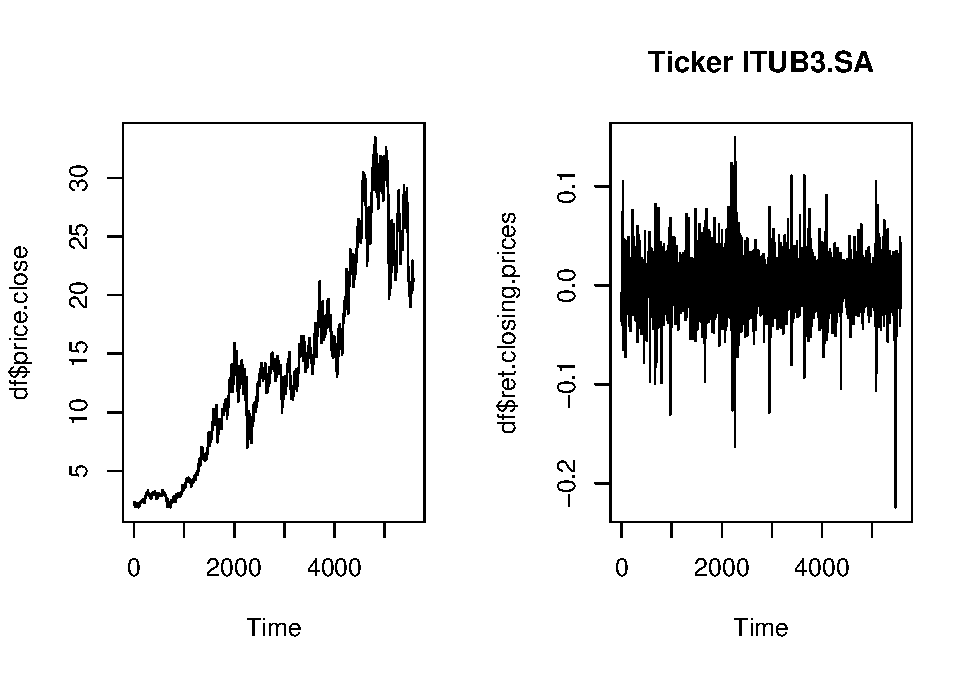
\includegraphics{work_files/figure-latex/unnamed-chunk-3-1.pdf}
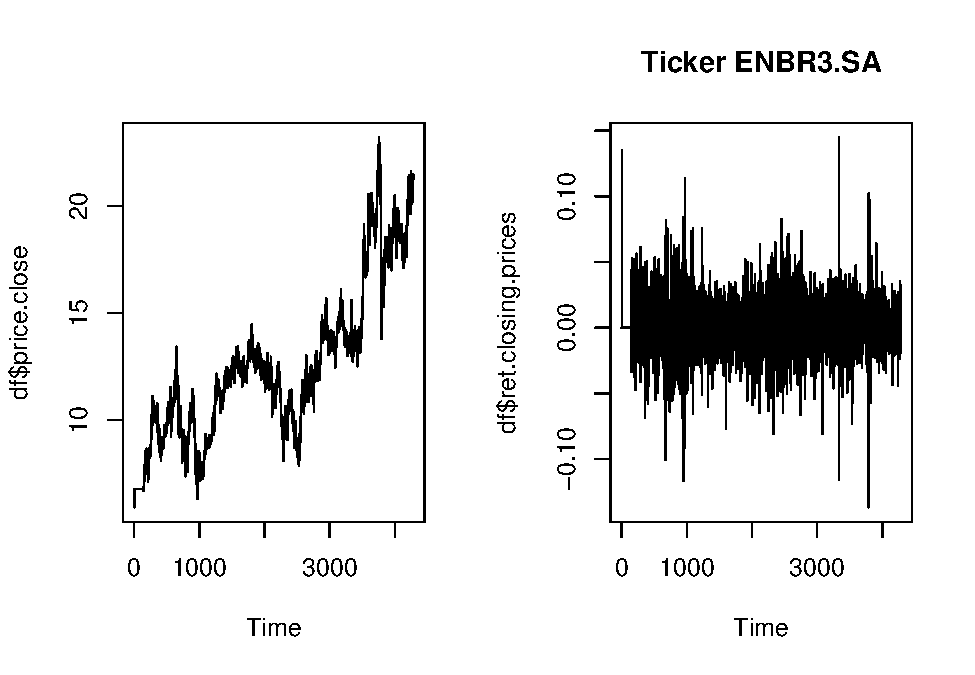
\includegraphics{work_files/figure-latex/unnamed-chunk-3-2.pdf}
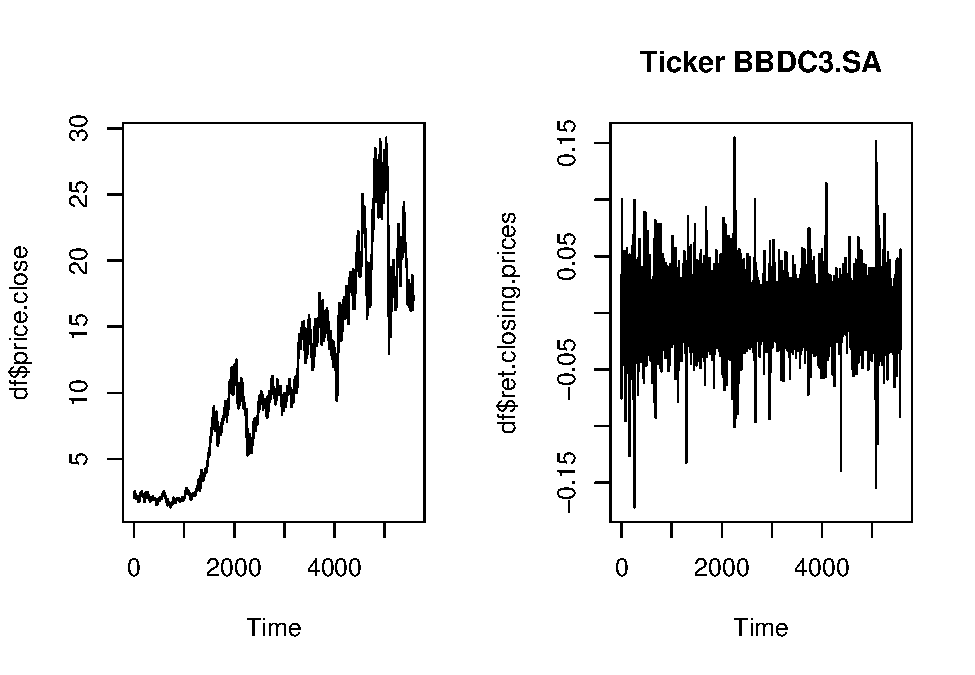
\includegraphics{work_files/figure-latex/unnamed-chunk-3-3.pdf}
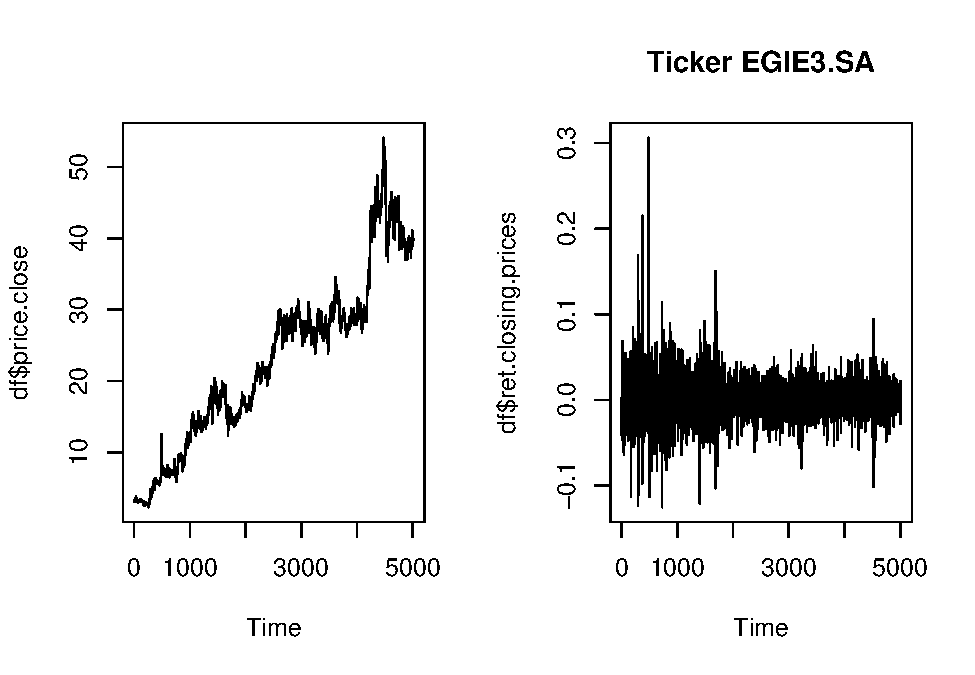
\includegraphics{work_files/figure-latex/unnamed-chunk-3-4.pdf}
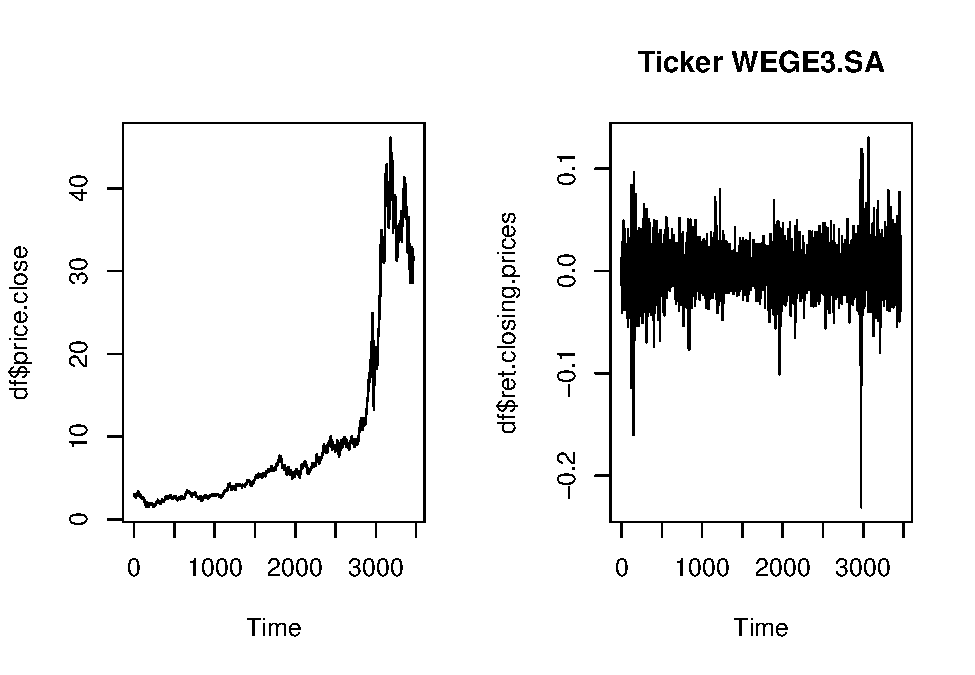
\includegraphics{work_files/figure-latex/unnamed-chunk-3-5.pdf}
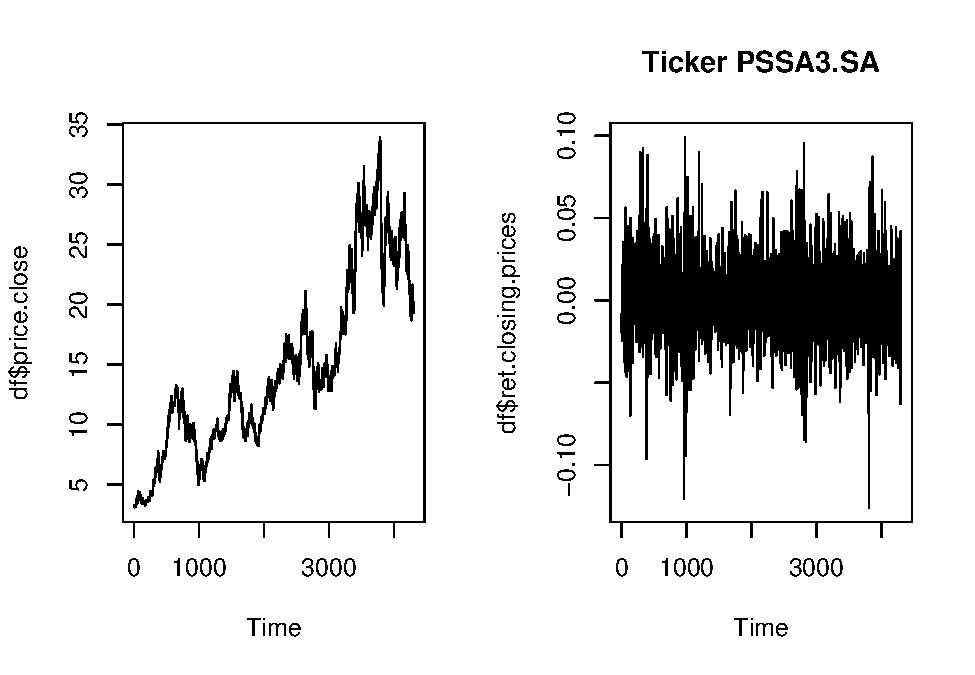
\includegraphics{work_files/figure-latex/unnamed-chunk-3-6.pdf}

\end{document}
